\chapter{IL-10-GAG interaction: evaluation of NMR data}
\section{Heparin structure models -- with and without presence of IL-10}

\begin{figure}
\centering
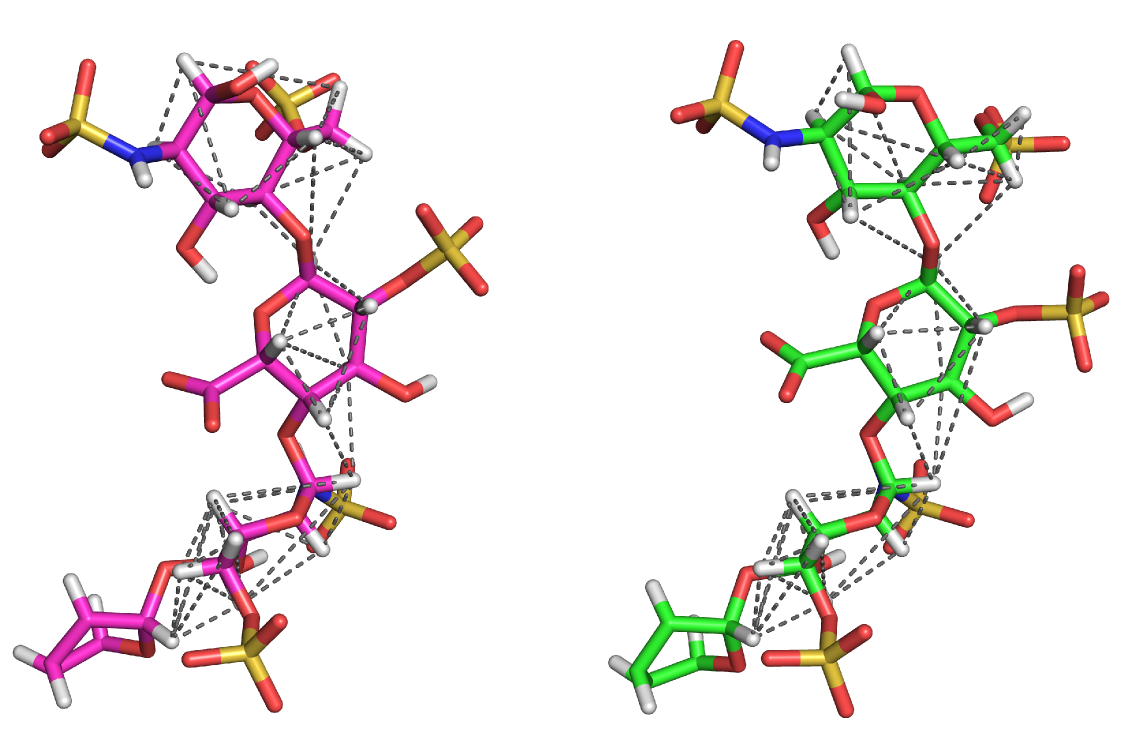
\includegraphics[width=0.9\textwidth]{gfx/nmr/two_cases_dashed_lines_distances.png}
\caption[]{
Heparin tetrasaccharide-internal H-H distance restraints applied during
simulated annealing MD simulations. Each dashed line corresponds to one NMR
distance restraint. In the unbound case (left, carbon in magenta), 42
restraints were applied. In the bound case (right, carbon in green), 41
restraints were used. Functional groups of ring A are not shown for clarity.
Atoms are color-coded with red, blue, yellow, gray corresponding to oxygen,
nitrogen, sulfur, and hydrogen, respectively.
}
\label{fig:nmr:hp_dashed_lines_distances}
\end{figure}



\begin{figure}
\centering
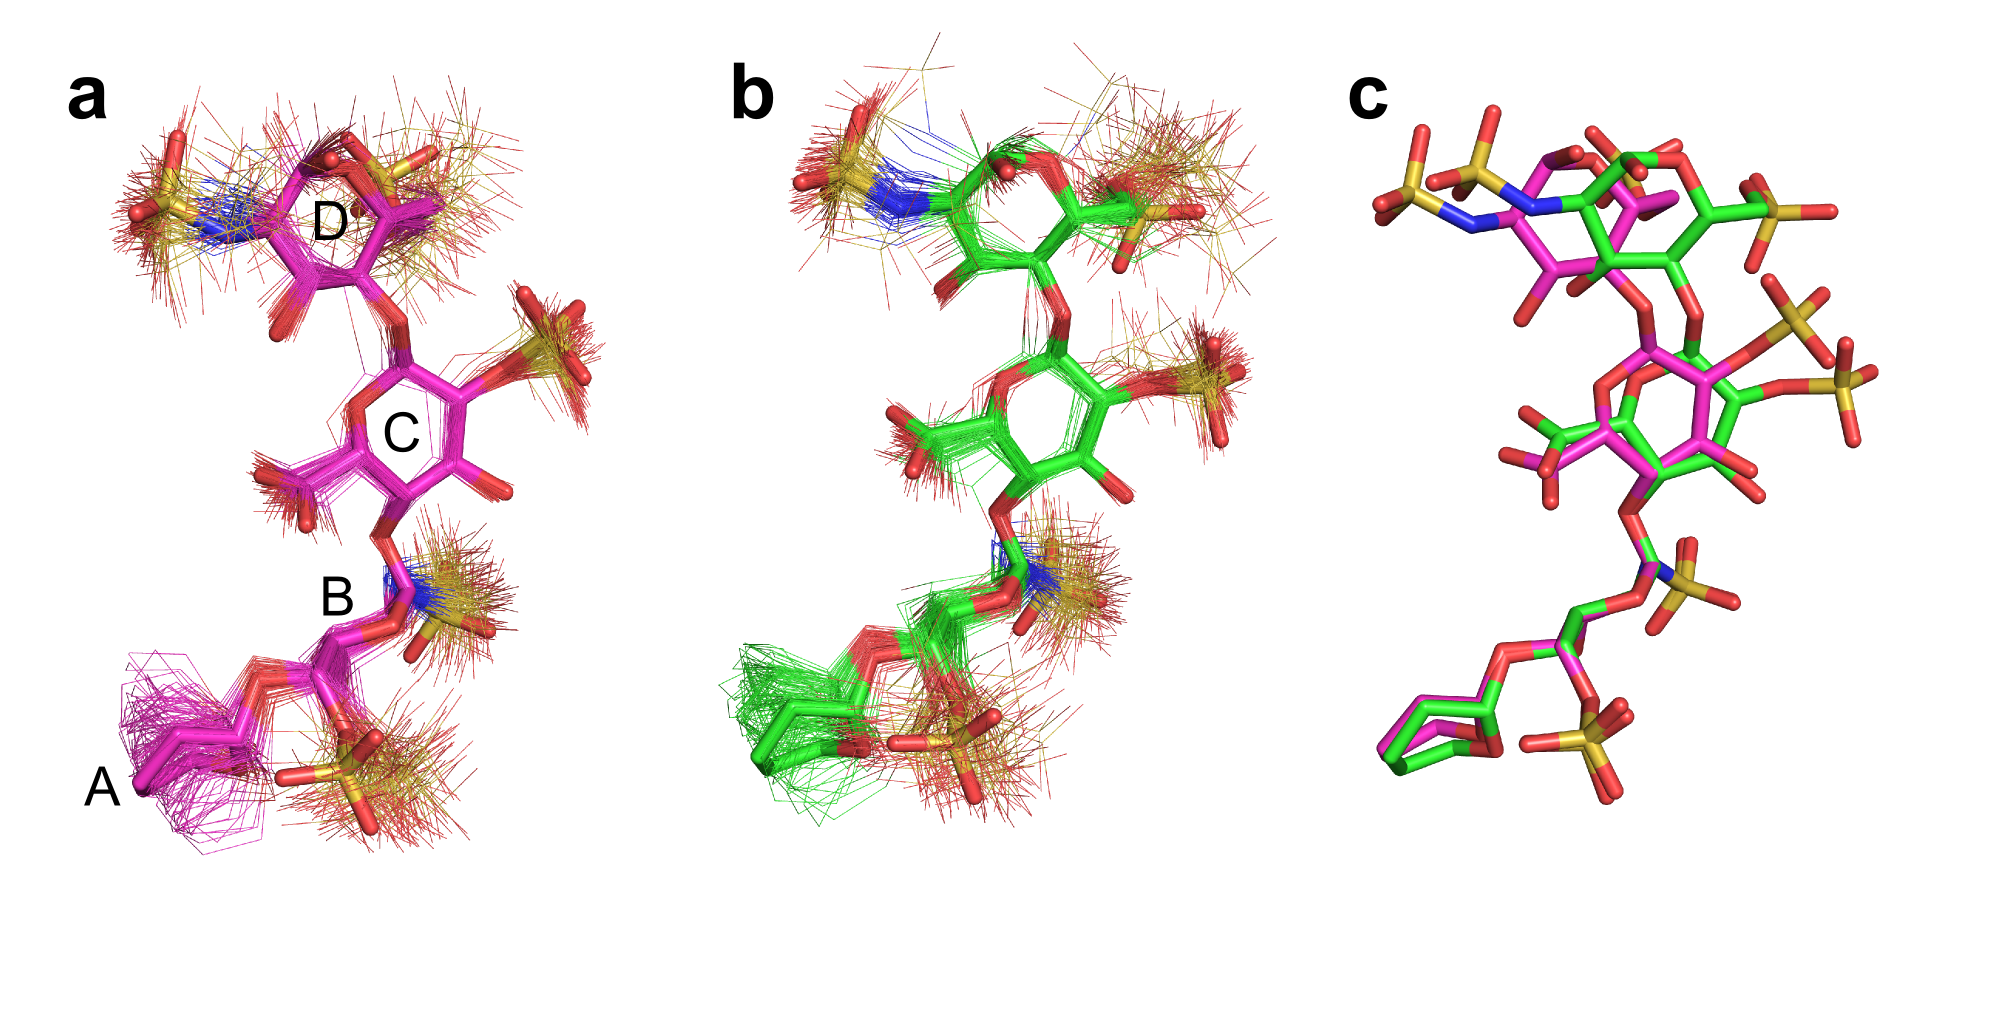
\includegraphics[width=0.9\textwidth]{gfx/nmr/Figure_07_bound_vs_free_three_panels_05.png}
\caption[]{
Heparin structure models obtained from NOE data and simulated annealing
simulations. (a) structure model ensemble for the unbound case (ring identifiers
in capital letters). (b) structure model ensemble for the bound case. (c) the
representative structure for both, the unbound (carbons in magenta) and bound
(carbons in green) ensembles, aligned on ring B. The ensemble representatives
are shown in thick sticks. Functional groups of ring A and hydrogens are not
shown for clarity. Atoms are colored by type (oxygen: red, nitrogen: blue,
sulfur: yellow).
}
\label{fig:nmr:hp_ensembles_representatives}
\end{figure}


\begin{figure}
\centering
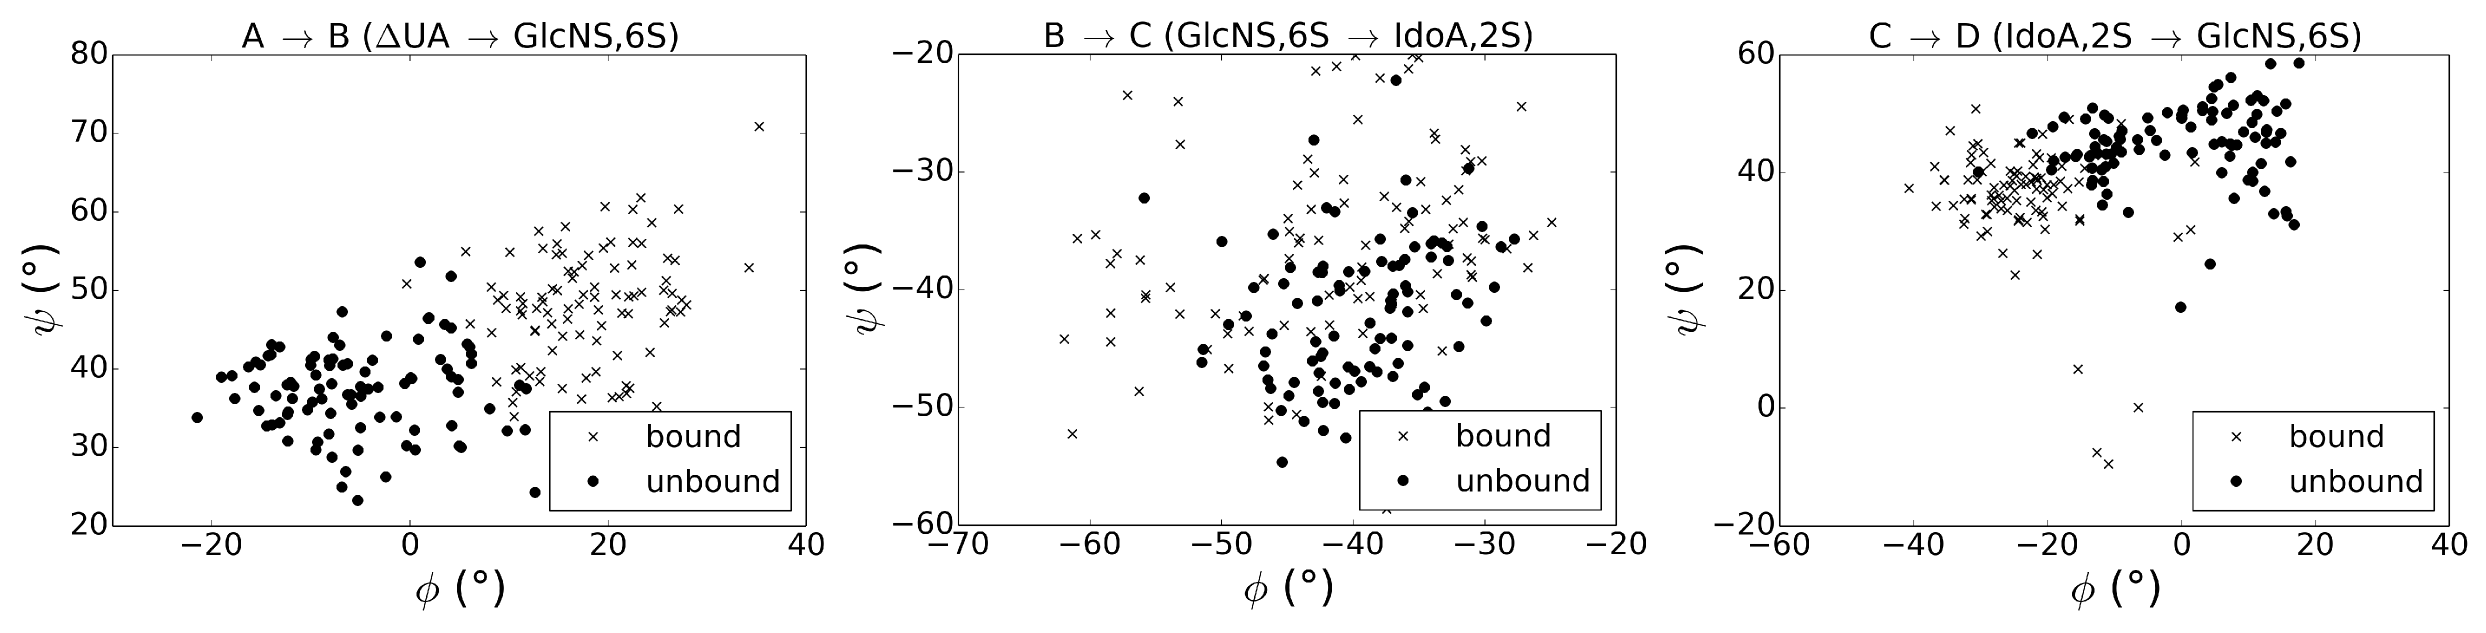
\includegraphics[width=0.9\textwidth]{gfx/nmr/Figure_08_glycolinkage_dihedrals_bound_vs_free_three_3panels_05.png}
\caption[]{
Glycosidic linkage torsional angle distributions of heparin structure model
ensembles obtained from NMR distance restraints and simulated annealing
simulations. Data comparing the bound and unbound state is shown individually
for each linkage in the heparin tetrasaccharide, namely for linkages A
\rightarrow B, B \rightarrow C, and C \rightarrow D.
}
\label{fig:nmr:hp_glyco_dihedral_distributions}
\end{figure}



\begin{figure}
\centering
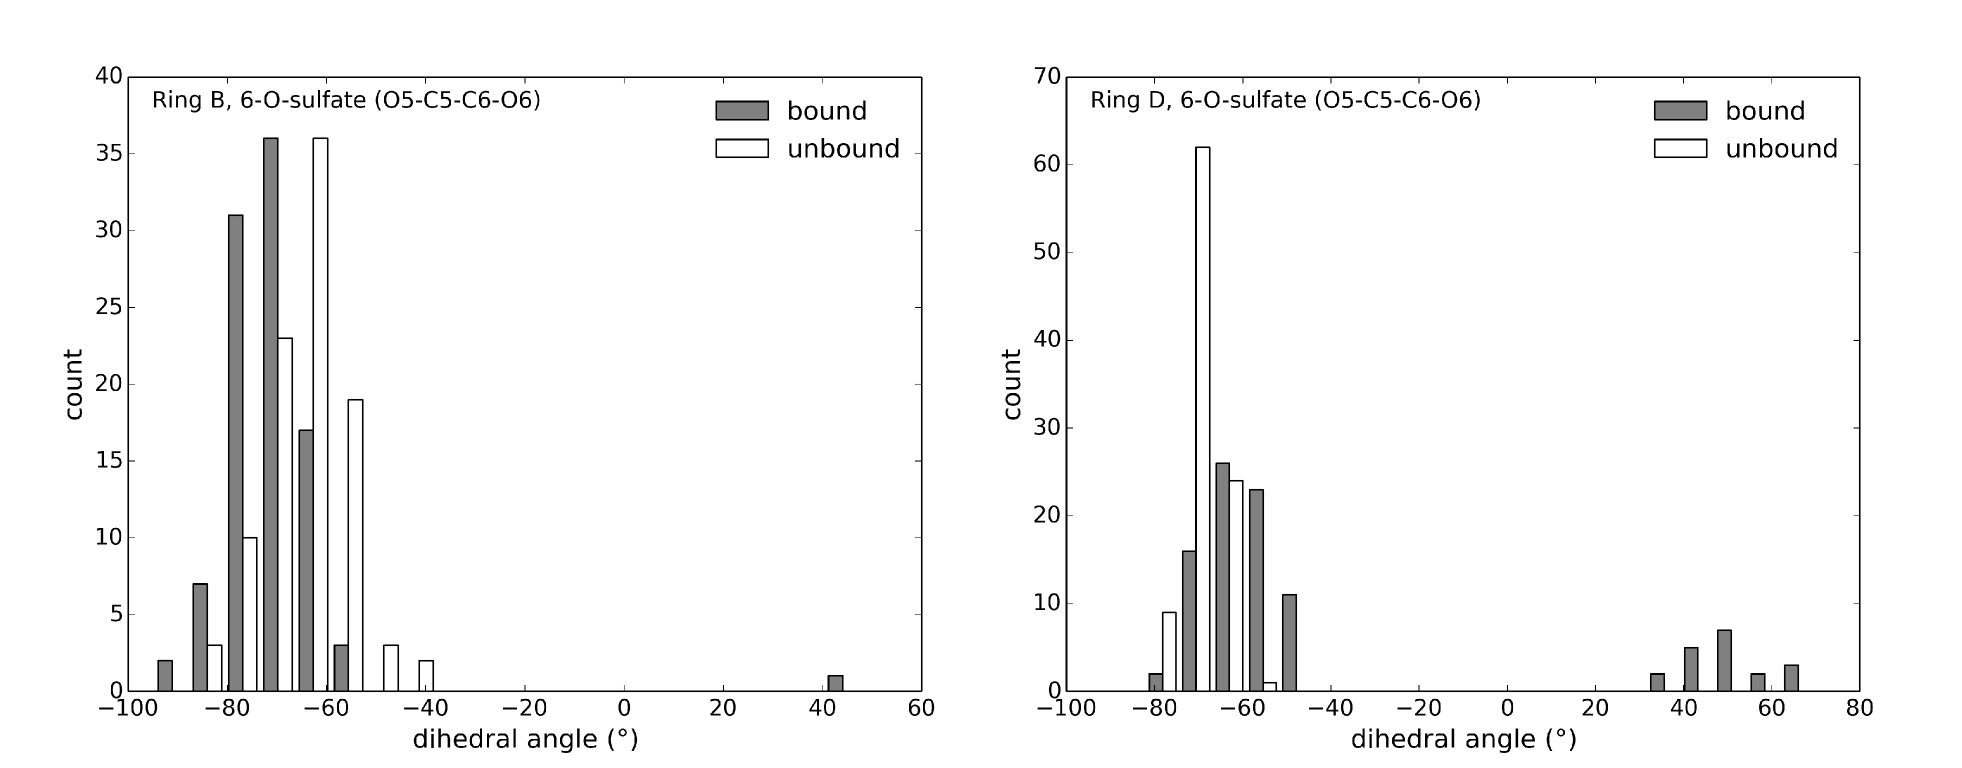
\includegraphics[width=0.9\textwidth]{gfx/nmr/SI_figure_6O_sulfate_dihedrals_B_D_01.png}
\caption[]{
Distribution of 6-O-sulfate orientations in heparin tetrasaccharide structure
models obtained from H-H NMR distance restraints and simulated annealing
simulations, in comparison for the bound and unbound state.
}
\label{fig:nmr:hp_sulfate_orientations}
\end{figure}






\section{Binding site determination via Pseudo Contact Shift measurements}
\hl{Should this be in the thesis? Maybe ONLY prediction would be better,
leave this for publication.}

\lipsum[1-5]